\documentclass[beamer,tikz,preview]{standalone}
% \includeonlyframes{currentf}
% \usepackage[T1]{fontenc}
\usepackage[utf8]{inputenc}
\usepackage[english]{babel}     
\usepackage{siunitx}
\usepackage{etoolbox}
\usepackage{listings}
\usepackage{color}
% ffmpeg -framerate 24 -i %04d.png qubit_projection.mp4
% ffmpeg -framerate 24 -start_number 94 -i %04d.png qubit_projection.mp4 
% \usepackage[]{qcircuit}


\usefonttheme[onlymath]{serif}

\newcommand*{\cB}{\mathcal{B}}
\newcommand*{\cC}{\mathcal{C}}
\newcommand*{\cD}{\mathcal{D}}
\newcommand*{\cE}{\mathcal{E}}
\newcommand*{\cF}{\mathcal{F}}
\newcommand*{\cG}{\mathcal{G}}
\newcommand*{\cH}{\mathcal{H}}
\newcommand*{\cI}{\mathcal{I}}
\newcommand*{\cM}{\mathcal{M}}
\newcommand*{\cN}{\mathcal{N}}
\newcommand*{\cP}{\mathcal{P}}
\newcommand*{\cQ}{\mathcal{Q}}
\newcommand*{\cR}{\mathcal{R}}
\newcommand*{\cS}{\mathcal{S}}
\newcommand*{\cT}{\mathcal{T}}
\newcommand*{\cU}{\mathcal{U}}
\newcommand*{\cV}{\mathcal{V}}
\newcommand*{\cW}{\mathcal{W}}
\newcommand*{\cX}{\mathcal{X}}
\newcommand*{\cY}{\mathcal{Y}}
\newcommand*{\cZ}{\mathcal{Z}}

\newcommand*{\id}{\mathrm{id}}
\newcommand*{\tr}{\mathrm{tr}}
\newcommand{\ket}[1]{\ensuremath{|#1\rangle}}
\newcommand{\bra}[1]{\ensuremath{\langle #1|}}
% \newcommand*{\ket}[1]{| #1 \rangle}
% \newcommand*{\bra}[1]{\langle #1 |}
\newcommand*{\spr}[2]{\langle #1 | #2 \rangle}
\newcommand*{\proj}[1]{|#1\rangle\!\langle #1|}

\newcommand*\xor{\mathbin{\oplus}}

\newcommand*{\eps}[0]{\varepsilon}
\newcommand*{\D}[0]{\mathbb{D}}
\newcommand*{\C}[0]{\mathbb{C}}
\newcommand*{\N}[0]{\mathbb{N}}
\newcommand*{\R}[0]{\mathbb{R}}
\newcommand*{\Z}[0]{\mathbb{Z}}

\newcommand{\cqubit}[1]{\raisebox{-.5\height}{\includegraphics[width=0.9cm]{figures/qubit_#1.png}}}
\newcommand{\cotimes}{\raisebox{-.5\height}{$\otimes$}}

\usepackage{multimedia}

\usepackage{cancel} % Barer des équations
\newcommand<>{\xxcancel}[1]{\alt#2{\xcancel{#1}\vphantom{#1}}{#1}}

\usepackage{tikz}
\usetikzlibrary{shapes.geometric,arrows,arrows.meta,shadows}
\usetikzlibrary{mindmap,backgrounds,positioning}
\usetikzlibrary{automata,positioning,fit,backgrounds}
\usetikzlibrary{positioning,arrows,matrix,calc,math}
\usepgflibrary{decorations.pathreplacing}
\usetikzlibrary{decorations.pathmorphing}
\usetikzlibrary{shapes.callouts}


\tikzset{my snake/.style={decorate,decoration={snake,amplitude=.4mm,segment length=2mm,post length=2mm}}}

\pgfdeclarelayer{background}
\pgfdeclarelayer{foreground}
\pgfsetlayers{background,main,foreground}   %% some additional layers for demo


\usetheme{Warsaw}
% \graphicspath{{pictures/}} % on change la racine des images

\usepackage [
  n,
  advantage,
  operators,
  sets,
  adversary,
  landau,
  probability,
  notions,
  logic,
  ff,
  mm,
  primitives,
  events,
  complexity,
  asymptotics,
  keys
  ] {cryptocode}

\renewcommand{\sample}[0]{\xleftarrow{\text{\tiny \$}}}

\usepackage[skins,many]{tcolorbox}
\newtcolorbox{subproof}{
  breakable,
  enhanced,
  frame hidden,
  interior hidden,
  opacityback=0,
  colframe=black,
  sharp corners,
  top = 0px, before skip = 0.1cm,
  bottom = 0px, after  skip = 0.1cm,  
  left=0.1cm, left skip=0.1cm,
  right=0px, right skip=0px,
  borderline west={0.02cm}{0pt}{black}
}

\usepackage{MyMnSymbol}

\definecolor{mygreen}{rgb}{0,0.6,0}
\definecolor{mygray}{rgb}{0.5,0.5,0.5}
\definecolor{mymauve}{rgb}{0.58,0,0.82}

\lstset{ %
  backgroundcolor=\color{white},   % choose the background color; you must add \usepackage{color} or \usepackage{xcolor}
  basicstyle=\footnotesize,        % the size of the fonts that are used for the code
  breakatwhitespace=false,         % sets if automatic breaks should only happen at whitespace
  breaklines=true,                 % sets automatic line breaking
  captionpos=b,                    % sets the caption-position to bottom
  commentstyle=\color{mygreen},    % comment style
  deletekeywords={...},            % if you want to delete keywords from the given language
  escapeinside={\%*}{*)},          % if you want to add LaTeX within your code
  extendedchars=true,              % lets you use non-ASCII characters; for 8-bits encodings only, does not work with UTF-8
  frame=single,	                   % adds a frame around the code
  keepspaces=true,                 % keeps spaces in text, useful for keeping indentation of code (possibly needs columns=flexible)
  keywordstyle=\color{blue},       % keyword style
  language=Octave,                 % the language of the code
  otherkeywords={*,...},           % if you want to add more keywords to the set
  numbers=left,                    % where to put the line-numbers; possible values are (none, left, right)
  numbersep=5pt,                   % how far the line-numbers are from the code
  numberstyle=\tiny\color{mygray}, % the style that is used for the line-numbers
  rulecolor=\color{black},         % if not set, the frame-color may be changed on line-breaks within not-black text (e.g. comments (green here))
  showspaces=false,                % show spaces everywhere adding particular underscores; it overrides 'showstringspaces'
  showstringspaces=false,          % underline spaces within strings only
  showtabs=false,                  % show tabs within strings adding particular underscores
  stepnumber=2,                    % the step between two line-numbers. If it's 1, each line will be numbered
  stringstyle=\color{mymauve},     % string literal style
  tabsize=2,	                   % sets default tabsize to 2 spaces
  title=\lstname                   % show the filename of files included with \lstinputlisting; also try caption instead of title
}

\newcommand{\includepdfpages}[1]{%
  \pdfximage{#1}%
  \foreach \ov in {1,...,\the\pdflastximagepages}{%
    \includegraphics<+>[page=\ov]{#1}%
  }%
}

\newcommand{\includepdfpageswidth}[2]{%
  \pdfximage{#2}%
  \foreach \ov in {1,...,\the\pdflastximagepages}{%
    \includegraphics<+>[page=\ov,width=#1]{#2}%
  }%
}

\newcommand{\includetikzpdfpageswidth}[3]{%
  \pdfximage{#2}%
  \foreach \ov in {1,...,\the\pdflastximagepages}{%
    \onslide<+>{\node[#3]{\includegraphics[page=\ov,width=#1]{#2}};}%
  }%
}

\newcommand{\includetikzpdfpages}[2]{%
  \pdfximage{#1}%
  \foreach \ov in {1,...,\the\pdflastximagepages}{%
    \onslide<+>{\node[#2]{\includegraphics[page=\ov]{#1}};}%
  }%
}

\newcommand{\includetikzpdfpageskeeplast}[2]{%
  \pdfximage{#1}%
  \pgfmathparse{\the\pdflastximagepages-1}
  \foreach \ov in {1,...,\pgfmathresult}{%
    \onslide<+>{\node[#2]{\includegraphics[page=\ov]{#1}};}%
  }%
  \onslide<+->{\node[#2]{\includegraphics[page=\the\pdflastximagepages]{#1}};}%
}

\newcommand{\tcancel}[1]{\ensuremath{\xcancel{\text{#1}}}}

%%% Local Variables:
%%% mode: latex
%%% TeX-master: t
%%% End:

\graphicspath{{../}}

\tikzset{my snake/.style={decorate,decoration={snake,amplitude=.4mm,segment length=2mm,post length=1mm}}}

\begin{document}
\begin{standaloneframe}
  \begin{tikzpicture}[ampersand replacement=\&,row sep=3mm,nodes={inner sep=0pt},
      qubit/.style={draw, circle, color=black, anchor=center,
        fill={rgb,255:red,143;green,146;blue,237},
        inner sep=0pt,minimum width=5mm},
      ]
    \matrix (m) {
      \node<1> {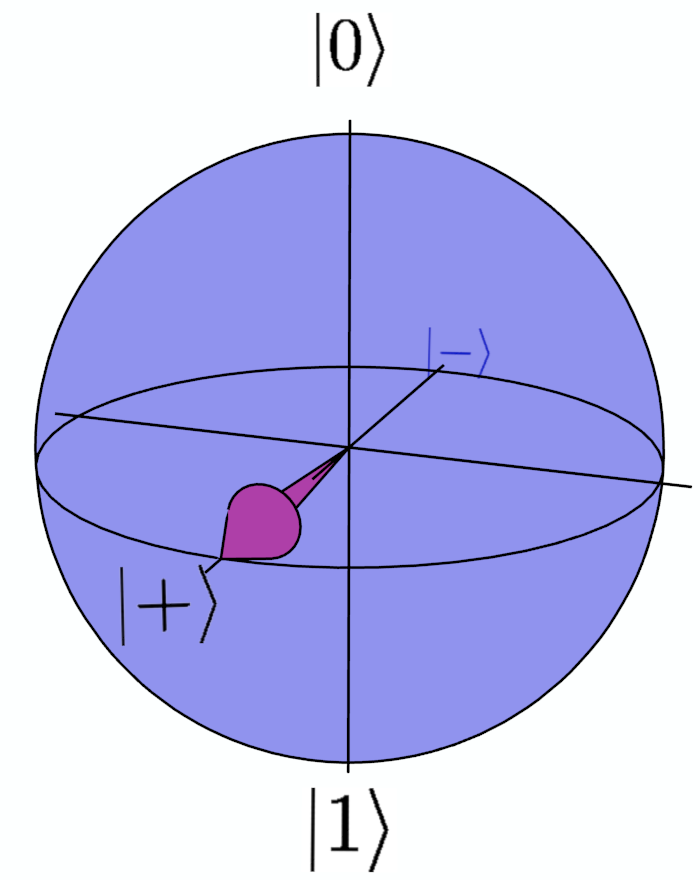
\includegraphics[width=.12\textwidth]{qubit_a0.png}}; \node<2-> {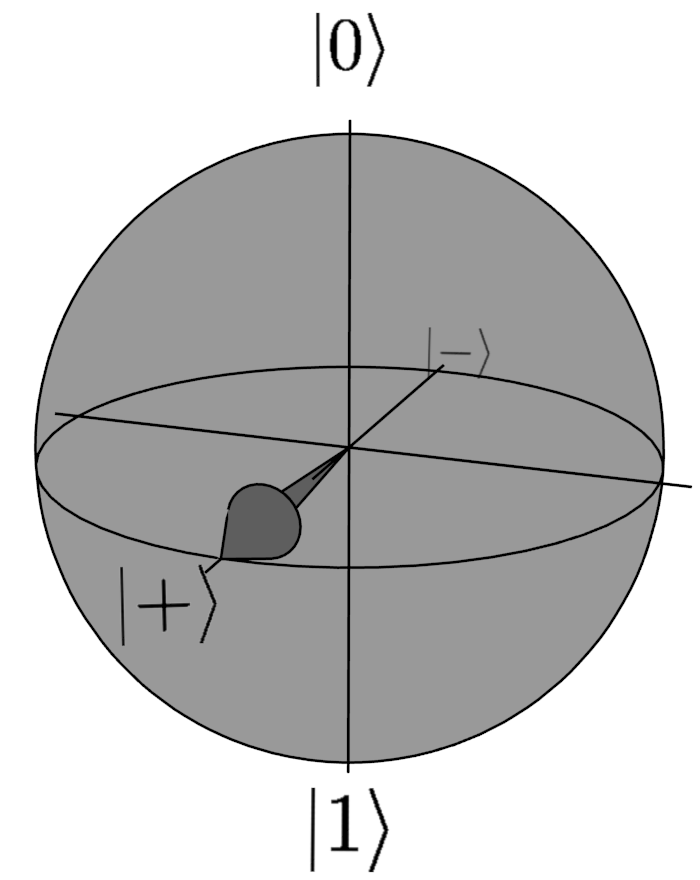
\includegraphics[width=.12\textwidth]{qubit_a0_grey.png}}; \&
      \node<1> {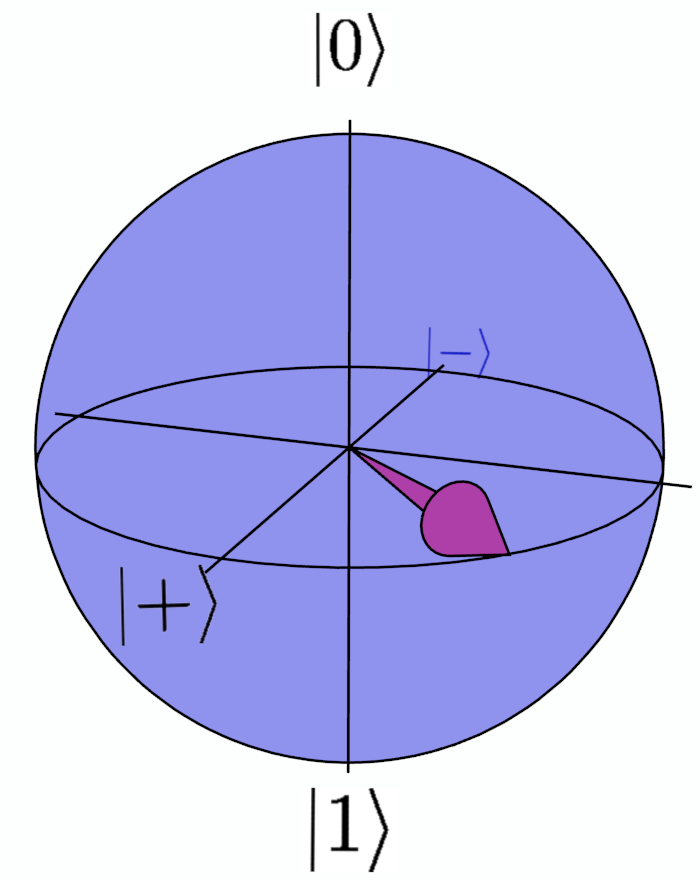
\includegraphics[width=.12\textwidth]{qubit_a1.png}}; \node<2-> {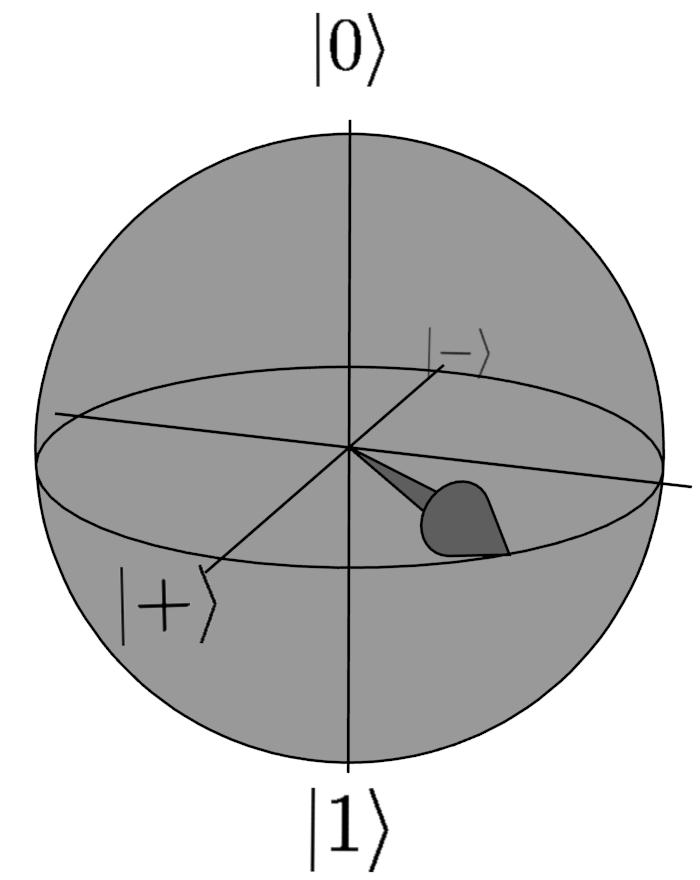
\includegraphics[width=.12\textwidth]{qubit_a1_grey.png}}; \&
      \node<1> {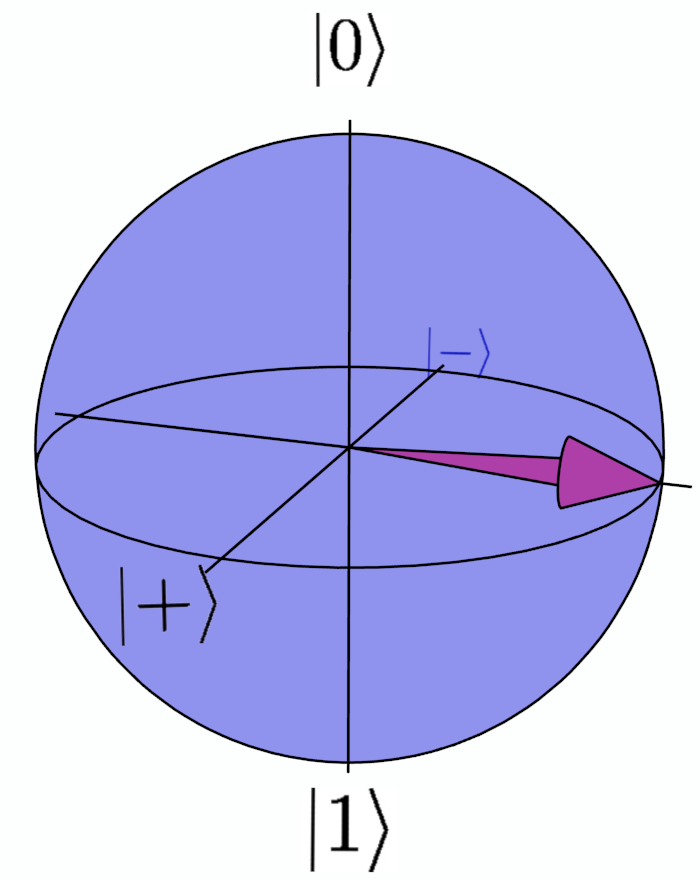
\includegraphics[width=.12\textwidth]{qubit_a2.png}}; \node<2-> {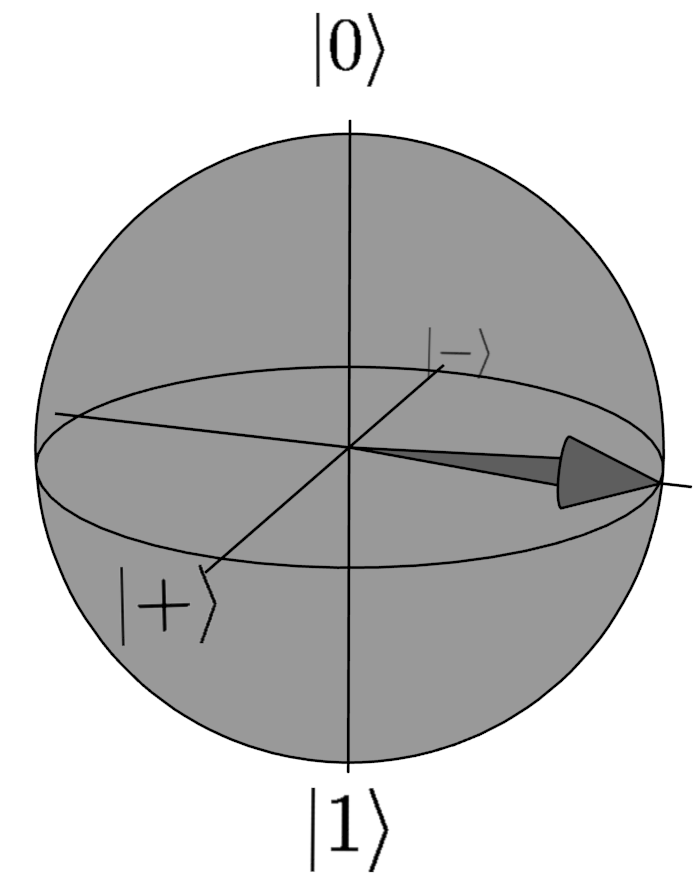
\includegraphics[width=.12\textwidth]{qubit_a2_grey.png}}; \&
      \node<1> {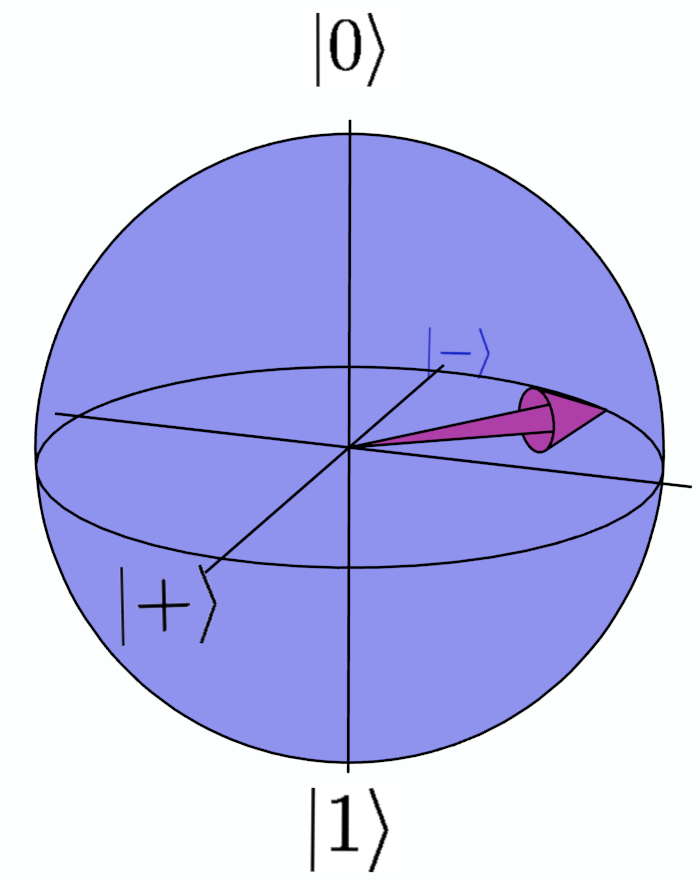
\includegraphics[width=.12\textwidth]{qubit_a3.png}}; \node<2-> {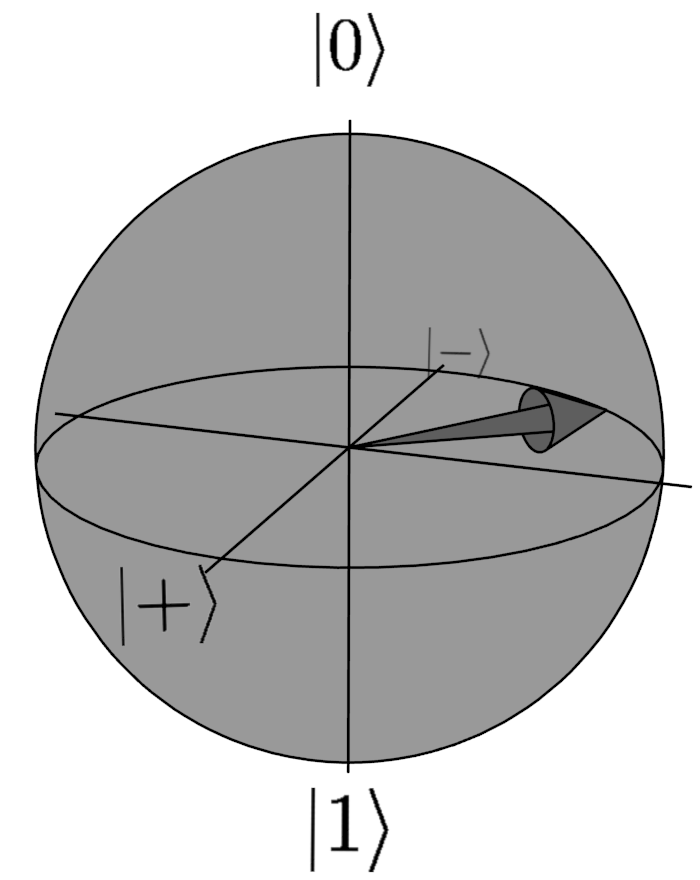
\includegraphics[width=.12\textwidth]{qubit_a3_grey.png}};  \node<5-> {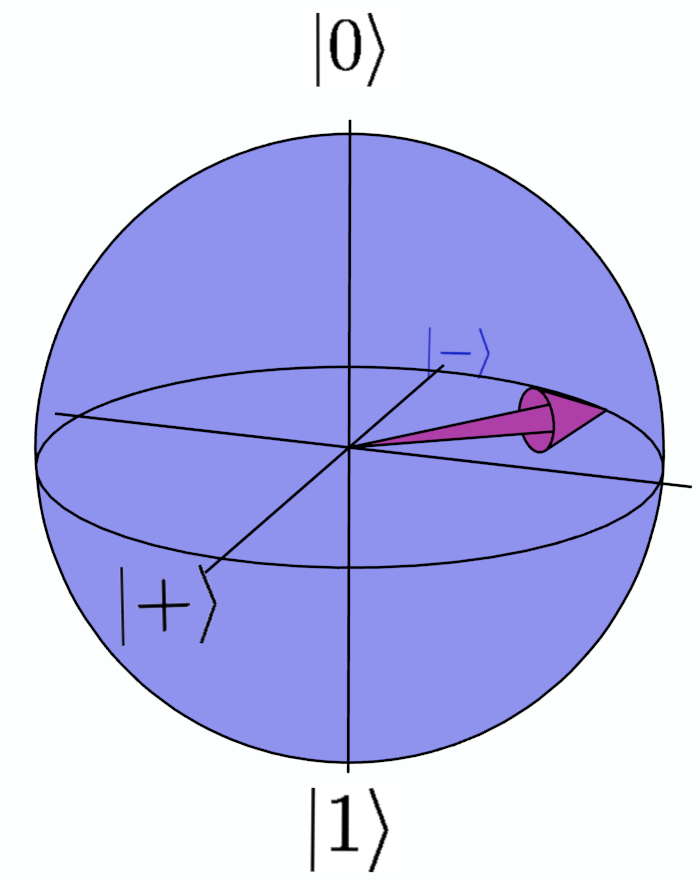
\includegraphics[width=.12\textwidth]{qubit_a3.png}}; \node<8-> {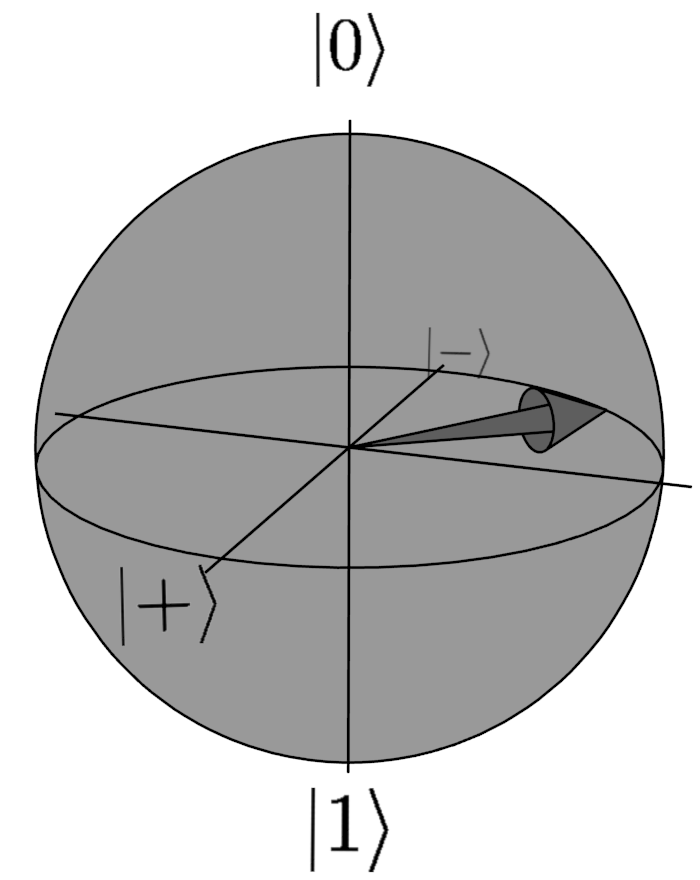
\includegraphics[width=.12\textwidth]{qubit_a3_grey.png}}; \\
      \node<1> {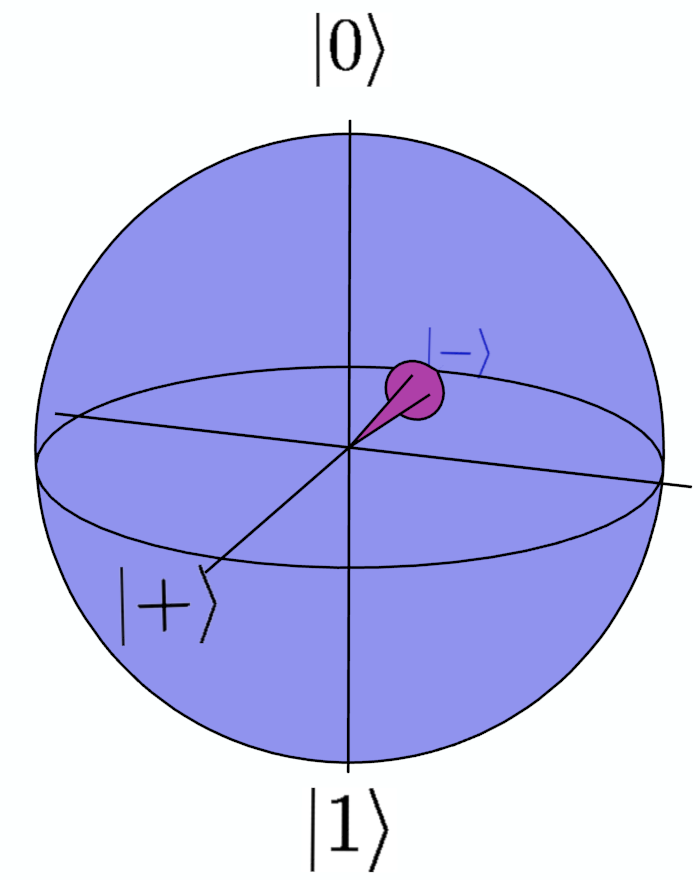
\includegraphics[width=.12\textwidth]{qubit_a4.png}}; \node<2-> {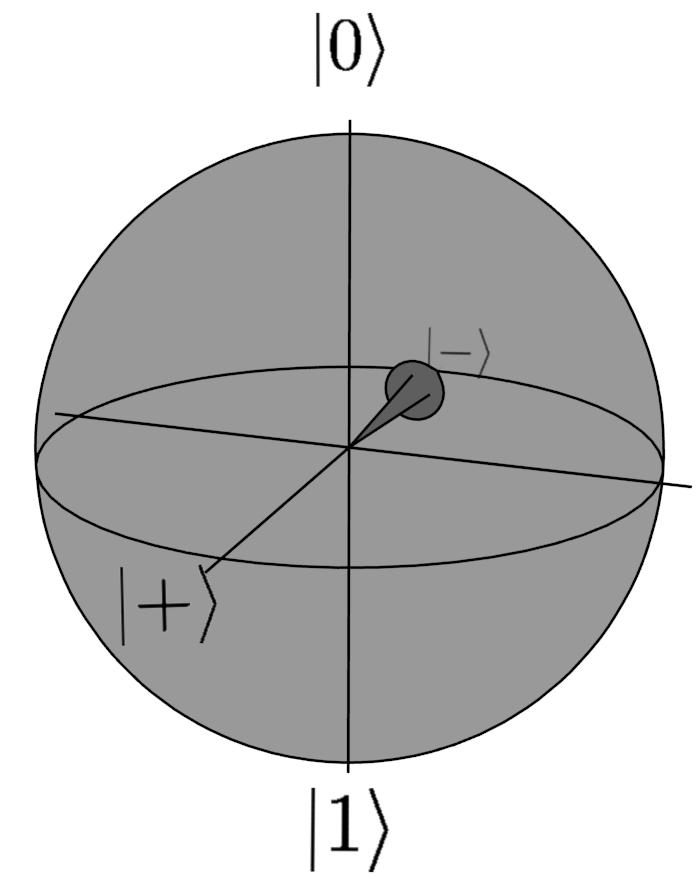
\includegraphics[width=.12\textwidth]{qubit_a4_grey.png}}; \&
      \node<1> {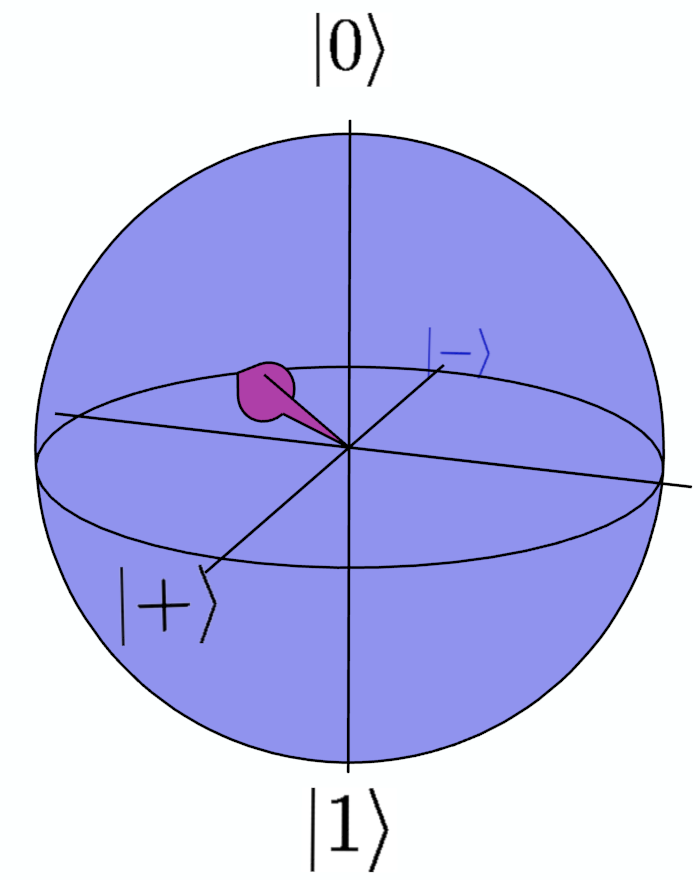
\includegraphics[width=.12\textwidth]{qubit_a5.png}}; \node<2-> {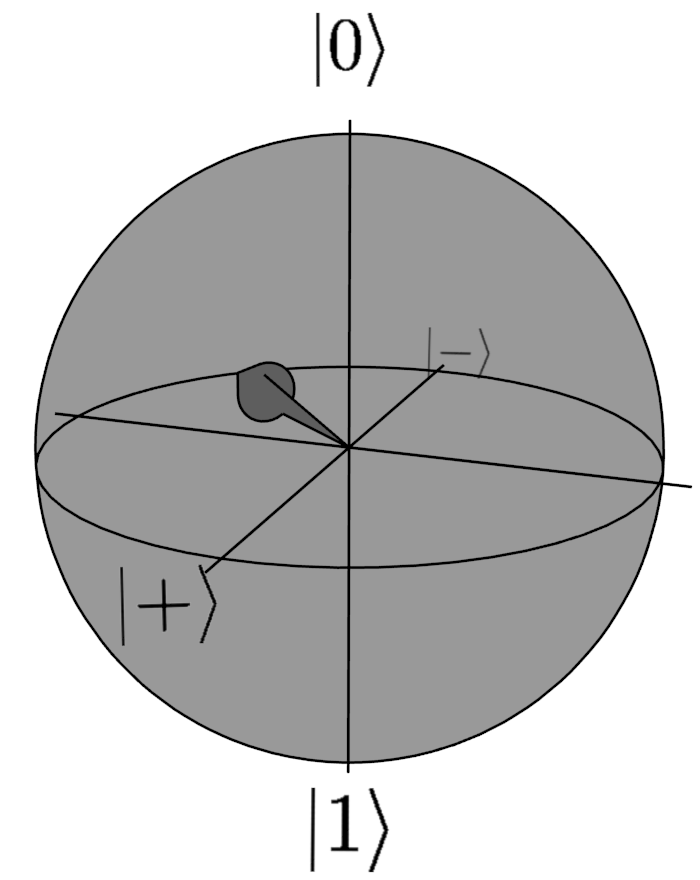
\includegraphics[width=.12\textwidth]{qubit_a5_grey.png}}; \&
      \node {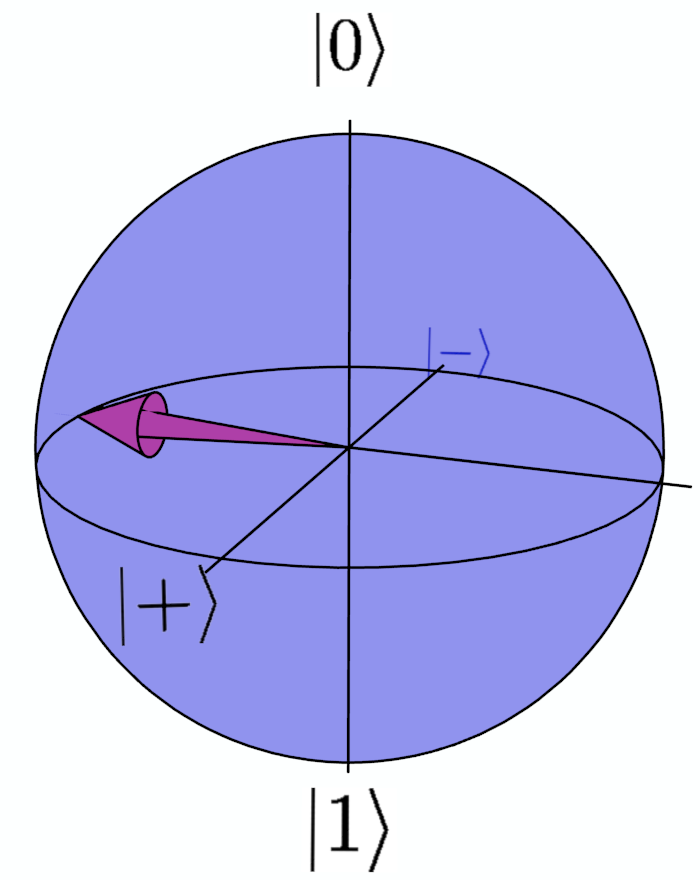
\includegraphics[width=.12\textwidth]{qubit_a6.png}}; \node<5-> {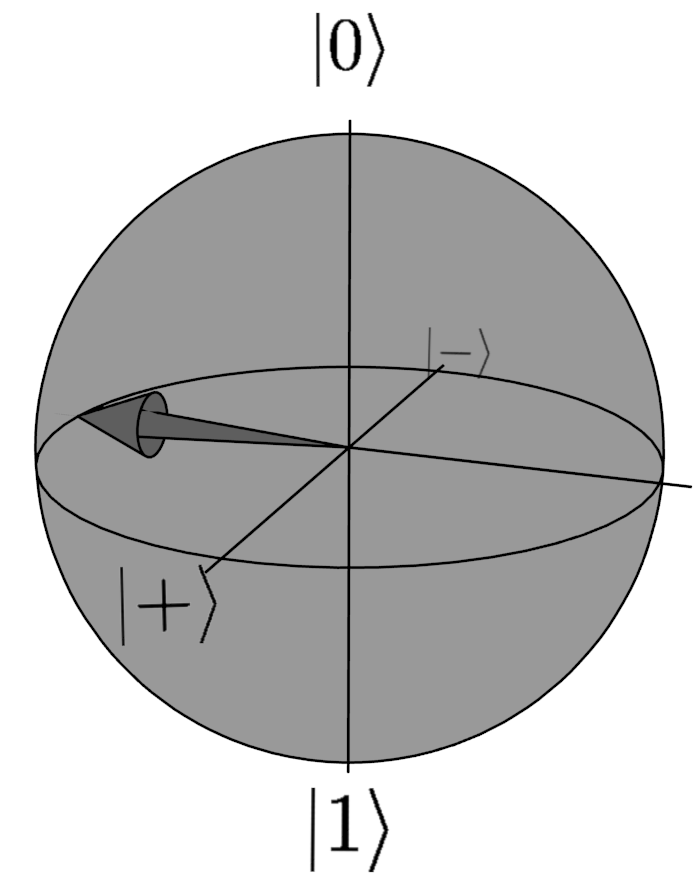
\includegraphics[width=.12\textwidth]{qubit_a6_grey.png}}; \&
      \node<1> {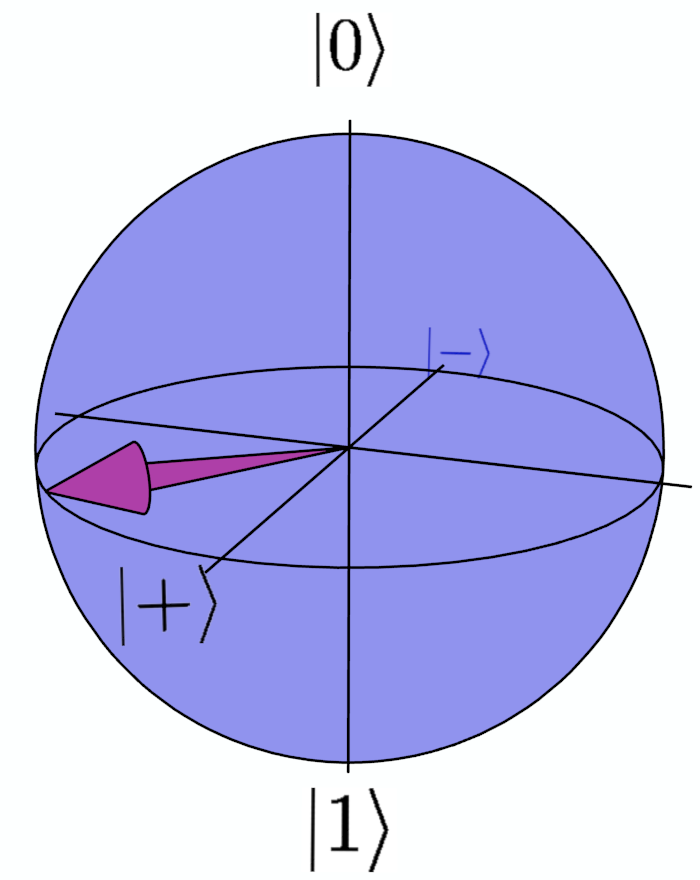
\includegraphics[width=.12\textwidth]{qubit_a7.png}}; \node<2-> {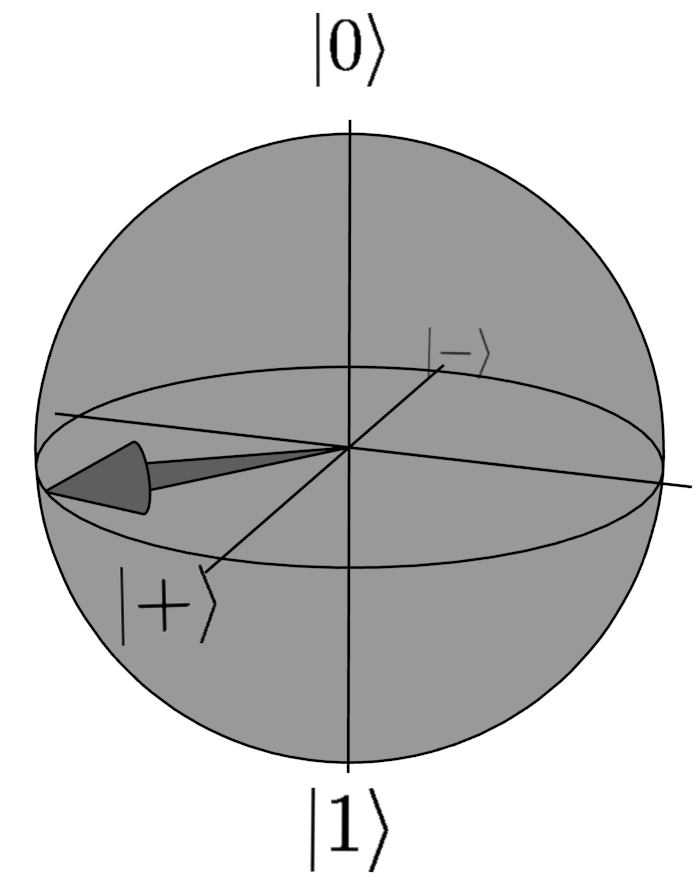
\includegraphics[width=.12\textwidth]{qubit_a7_grey.png}}; \\
    };
    % Alice
    \node[inner sep=0pt, below= 3mm of m](alice) {
\includegraphics[width=.20\textwidth]{aliceteacup.png}};
    % Bob
    \node[inner sep=0pt,right=.50\textwidth of alice](bob) {
\includegraphics[width=.20\textwidth]{bob_marley_aveugle.jpg}};
    % Flèches
    % \draw<3->[-latex] ([yshift=.04\textwidth]alice.east) -- ([yshift=.04\textwidth]bob.west |- alice.west);
    \draw<12>[-latex] ([yshift=-.04\textwidth]bob.west |- alice.west) -- ([yshift=-.04\textwidth]alice.east);
    % Flèche logo atome
    \draw<3-4>[-latex,my snake] ([yshift=.04\textwidth]alice.east) -- ([yshift=.04\textwidth]bob.west |- alice.west) node[midway,above=2mm] {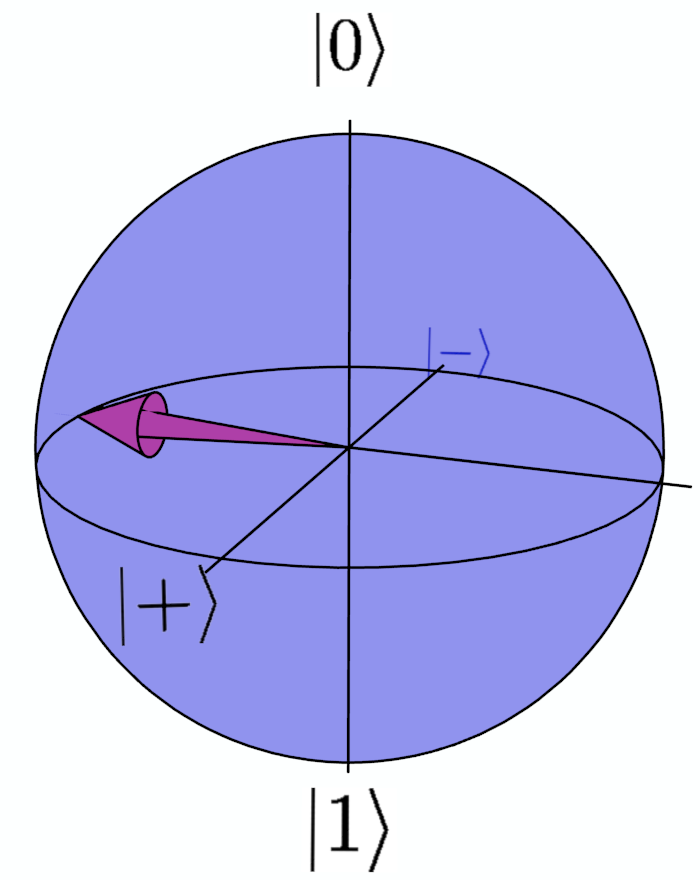
\includegraphics[width=.12\textwidth]{qubit_a6.png}};
    \draw<6-7>[-latex,my snake] ([yshift=.04\textwidth]alice.east) -- ([yshift=.04\textwidth]bob.west |- alice.west) node[midway,above=2mm] {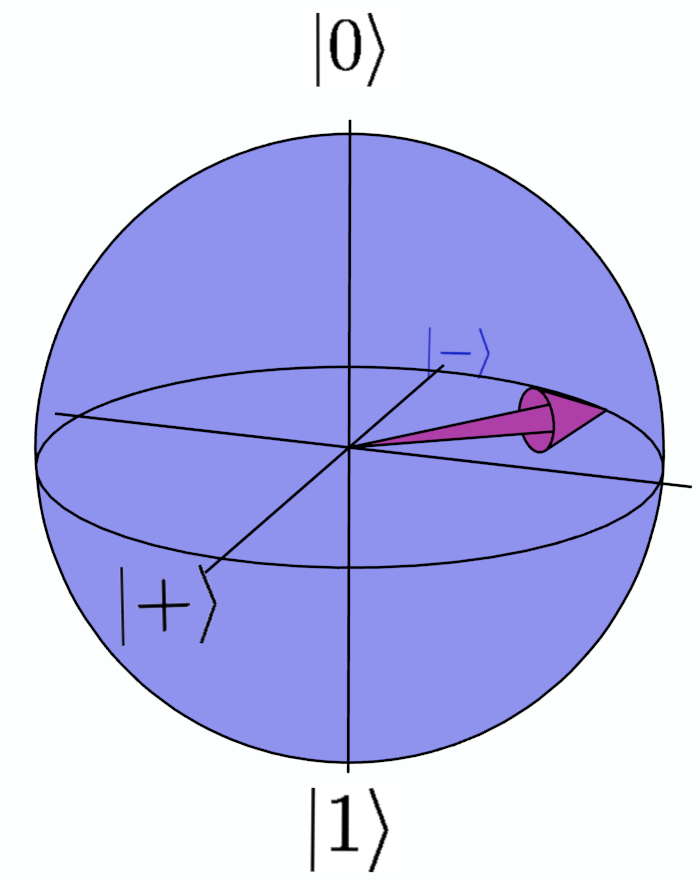
\includegraphics[width=.12\textwidth]{qubit_a3.png}};
    \draw<9-10>[-latex] ([yshift=.04\textwidth]alice.east) -- ([yshift=.04\textwidth]bob.west |- alice.west);
    % 
    % Graph
    \node[above=1.5cm of bob.north east, anchor=south east] (graph) {
      \begin{tikzpicture}[scale=0.5, every node/.style={transform shape},
          line qubit/.style={-{Stealth[scale=.5]}},
          pacman/.pic={
            \fill[yellow] (-5mm,0) -- ++ (45:5mm) arc (45:315:5mm) -- (-5mm,0);
            \fill[black] (-5mm,0) ++ (90:3mm) circle (.7mm);
          },
          dashed pacman/.pic={
            \fill[yellow!50] (-5mm,0) -- ++ (45:5mm) arc (45:315:5mm) -- (-5mm,0);
            \draw[black,dashed] (-5mm,0) -- ++ (45:5mm) arc (45:315:5mm) -- (-5mm,0);
            \fill[black] (-5mm,0) ++ (90:3mm) circle (.7mm);
          }
          ]
        \tikzmath{
          int \x, \y;
          int \xmax, \ymax, \xp, \yp;
          \xmax = 10;
          \ymax = 3;
          %%%% Draw brickwork
          %% Invisible Nodes
          for \x in {0,...,\xmax}{
            for \y in {0,...,\ymax}{
              {\coordinate(n-\x-\y) at (\x,\y);};
            };
          };
          %% Horizontal lines
          for \x in {1,...,\xmax-1}{
            for \y in {0,...,\ymax}{
              \xp = \x + 1;
              {\draw (n-\x-\y.center) -- (n-\xp-\y.center);};
            };
          };
          %% Vertical lines
          for \x in {0,...,\xmax}{
            for \y in {0,...,\ymax-1}{
              if (Mod(\y,2) == 0 && (Mod(\x,9) == 2 || Mod(\x,9) == 4)) || (Mod(\y,2) == 1 && \x > 1 && (Mod(\x,9) == 6 || Mod(\x,9) == 8)) then {
                \yp = \y + 1;
                {\draw (n-\x-\y) -- (n-\x-\yp);};
              };
            };
          };
          %% Nodes
          for \x in {1,...,\xmax}{
            for \y in {0,...,\ymax}{
              {
                \node[qubit,fill=white] (m-\x-\y) at (n-\x-\y){};
              };
            };
          };
          %% Blue nodes
          {
            \onslide<4->{
              \node[qubit] (q1) at (n-1-3){};
              \draw[red,line qubit] (q1.center) -- (q1.east);
            }
            \onslide<7->{
              \node[qubit] (q1) at (n-1-2){};
              \draw[red,line qubit] (q1.center) -- (q1.south west);
            }
            \onslide<8->{
              \pgfmathsetseed{1}
              % First column
              \node[qubit] (q1) at (n-1-1){};
              \draw[red,line qubit] (q1.center) -- (q1.north);
              \node[qubit] (q1) at (n-1-0){};
              \draw[red,line qubit] (q1.center) -- (q1.north west);
              % Other columns
              \pgfmathdeclarerandomlist{randomanchors}{{north}{north east}{east}{south east}{south}{south west}{west}{north west}}
              \foreach \x in {2,...,\xmax}{
                \foreach \y in {0,...,\ymax}{
                  \node[qubit] (q1) at (n-\x-\y){};
                  \pgfmathrandomitem{\myanchor}{randomanchors}
                  \draw[red,line qubit] (q1.center) -- (q1.\myanchor);
                }
              }
            }
            %% Pacmans !
            \onslide<9>{
              \pic at (n-1-3) {dashed pacman};
            }
            \onslide<10>{
              \pic[rotate=-90] at (n-1-3) {pacman};
            }
            \onslide<11->{
              \node[qubit,fill=yellow] at (n-1-3){};
            }
            \onslide<13->{
              \foreach \x in {1,...,\xmax}{
                \foreach \y in {0,...,\ymax}{
                  \node[qubit,fill=yellow] (q1) at (n-\x-\y){};
                }
              }
              \foreach \y in {0,...,\ymax}{
                \node[qubit] (q1) at (n-\xmax-\y){};
              }
            }
            \onslide<14>{
              \foreach \y in {0,...,\ymax}{
                \node[qubit,fill=yellow] (q1) at (n-\xmax-\y){};
              }
            }
          };
        }
      \end{tikzpicture}
    };
    % \node[fill=green,inner sep=0pt,minimum size=3pt] at (graph.north east) {};
    % \node[fill=red,inner sep=0pt,minimum size=3pt] at (graph.north west) {};
    % \node[fill=yellow,inner sep=0pt,minimum size=3pt] at (graph.south east) {};
    % \node[fill=orange,inner sep=0pt,minimum size=3pt] at (graph.south west) {};
  \end{tikzpicture}
\end{standaloneframe}
\end{document}

%%% Local Variables:
%%% mode: latex
%%% TeX-master: t
%%% End:
